\subsubsection{Editar}

  \paragraph{}Para editar un elemento del sistema, es necesario pulsar el
  icono \textit{Editar}. Se puede ver una captura de pantalla de este
  icono en la figura \ref{capturaEditElemento}. También es posible acceder
  al formulario de edición del elemento pulsando sobre el nombre del elemento
  que aparece en el listado.

  \paragraph{}Al pulsar en el icono, se enlazará con el formulario de edición
  del elemento. Este formulario se puede ver en la imagen
  \ref{capturaEditReunionPreguntaAsesor}.

  \begin{figure}[!ht]
    \begin{center}
      \fbox{
      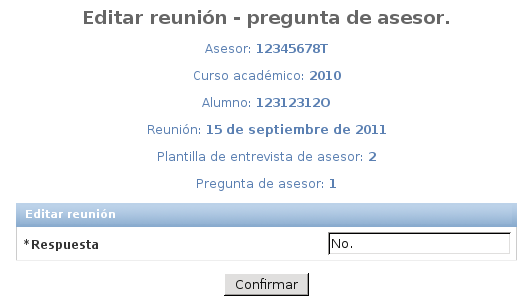
\includegraphics[scale=0.55]{4.Funcionamiento_Aplicacion/4.3.Gestion/4.3.1.Administrador_Principal/4.3.1.16.Reunion_PreguntaAsesor/edit_reunion_preguntaAsesor.png}
      }
      \caption{Captura de pantalla del formulario de edición de \textit{Reunión - Pregunta de asesor}.}
      \label{capturaEditReunionPreguntaAsesor}
    \end{center}
  \end{figure}

  \paragraph{}Una vez rellenado el formulario, se pulsará el botón
  \textit{Confirmar}, el cual se puede ver en la figura
  \ref{capturaBotonConfirmar}. Si el formulario rellenado es válido, y no tiene
  errores, se editará la información del elemento en el sistema. En caso de
  contener información no válida, un mensaje de error aparecerá indicando los
  campos del formulario que no han pasado la validación, los cuales habrá que
  corregir para modificar correctamente el elemento en el sistema.
